\documentclass[a4paper,12pt]{article} % тип документа


\usepackage[T2A]{fontenc} % кодировка
\usepackage[utf8]{inputenc} % кодировка исходного текста
\usepackage[english,russian]{babel} % локализация и переносы

% colors
\usepackage[dvipsnames,table,xcdraw]{xcolor}          
\definecolor{light-blue}{rgb}{0.8,0.85,1}


%symbols
\usepackage{upgreek}
\usepackage{amsmath,amsfonts,amssymb,amsthm,mathtools} %math
% теоремы
\theoremstyle{plain}
\newtheorem{definition}{Определение}[section] 
\newtheorem{theorem}{Теорема}
\newtheorem{example}{Пример}
\numberwithin{equation}{section}



% гиперссылки:
\usepackage{hyperref}
\definecolor{darkblue}{HTML}{0000A0}
\definecolor{linkcolor}{HTML}{0000FF}
\hypersetup{pdfstartview=FitH, citecolor=linkcolor, linkcolor=darkblue,urlcolor=red, colorlinks=true}


% графика:
\usepackage{graphics}
\graphicspath{{pic/}}
\DeclareGraphicsExtensions{.pdf,.png,.jpg, .eps}
\usepackage{caption} % а что без этого летит? (забыл)
\usepackage[section,above,below]{placeins} % управление плавающими объектами (?)
\usepackage{floatflt}
\usepackage{framed}



% работа с таблицами (?)
\usepackage{multirow}
\newcommand{\specialcell}[2][c]{%
	\begin{tabular}[#1]{@{}c@{}}#2\end{tabular}} % перенос строки в ячейке таблицы при пакете multirow


\newcommand{\comment}[1]{} % for multiline comments

% defining red box
\newsavebox{\selvestebox}
\newenvironment{colbox}[1]
{\newcommand\colboxcolor{#1}%
	\begin{lrbox}{\selvestebox}%
		\begin{minipage}{\dimexpr\columnwidth-2\fboxsep\relax}}
		{\end{minipage}\end{lrbox}%
	\begin{center}
		\colorbox[HTML]{\colboxcolor}{\usebox{\selvestebox}}
\end{center}}

% предметный указатель и библиография
\usepackage{makeidx}
\makeindex
\usepackage[nottoc]{tocbibind}

% разметка и стиль (???)
\usepackage[left=2cm, right=2cm, top=2cm, bottom=2cm]{geometry}
\usepackage{fancyhdr}
\pagestyle{fancy}
\fancyhead[L]{\rightmark}
%\lhead{ краткое название}
\chead{}
\rhead{\thepage}
\cfoot{} % get rid of the page number 
\renewcommand{\headrulewidth}{1pt}
\renewcommand{\footrulewidth}{0pt}
\usepackage{indentfirst}

\usepackage{framed}
\usepackage{fancyvrb} %for fraim aroun verbatim
 % основная шапка


\author{Юрий Голубев\\ yura.winter@gmail.com }
\title{Задание по квантовой теории поля}
\date{\today}

\usepackage{cancel}
\usepackage{float}


\newcommand{\parder}[2]{\frac{\partial {#1}}{\partial {#2}}} % в самом деле, это удобно.

\usepackage{bbm}

\begin{document}
\maketitle

\begin{abstract}
квантовая теория поля
\end{abstract}
%%%%%%%%%%%%%%%%%%%%%%%%%%%%%%%%%%%%%%%%%%%%%%%%%%%%%%%%%%%%%%	
\tableofcontents


\section*{Предисловие}
\addcontentsline{toc}{section}{Предисловие}

тренируемся, практикуемся


















\clearpage
\part{Первое задание}


\section{упражнения}


\begin{task}\textbf{1}

Рассмотреть вещественный 4-вектор в представлении группы Лоренца $\left(\frac{1}{2}, \frac{1}{2}\right)$



Рассмотрим произвольную эрмитово сопряженную величину
$\hat{V}$ в представлении 
$\left(\frac{1}{2}, \frac{1}{2}\right)$.


$\hat{V}$ несет пару индексов $\{\alpha \dot{\alpha}\},$ 
может быть разложена по базису матриц $\sigma^{\nu}:$
$$
(\hat{V})_{\alpha \dot{\alpha}}
=
\sigma_{\alpha \dot{\alpha}}^{\nu} V_{\nu}
$$
причем
$$
V^{\mu}
=
\frac{1}{2} \operatorname{tr}\left\{\bar{\sigma}^{\mu} \hat{V}\right\}
=
\frac{1}{2} \operatorname{tr}\left\{\hat{V} \bar{\sigma}^{\mu}\right\}
$$
так как по определению в (1.58) и (1.59), очевидно, 
что антисимметричная по пространственным индексам часть произведения матриц не дает вклада в след, 
ввиду бесследовости обычных 3 -мерных матриц Паули,
$$
\operatorname{tr}\left\{\bar{\sigma}^{\mu} \sigma^{\nu}\right\}=2 g^{\mu \nu}
$$


Согласно установленным нами законам преобразования верхних и нижних спинорных индексов, 
преобразования группы $\mathrm{SL}(2, \mathbb{C})$ переводят $\hat{V}$ в эрмитову величину
$$
\hat{V}^{\prime}=\Lambda_{-} \hat{V} \Lambda_{-}^{\dagger}
$$
которая опять может быть разложена по исходному базису релятивистских матриц Паули:
$$
V^{\prime \mu}=
\frac{1}{2} \operatorname{tr}\left\{\bar{\sigma}^{\mu} \hat{V}^{\prime}\right\}=
\frac{1}{2} \operatorname{tr}\left\{\hat{V}^{\prime} \bar{\sigma}^{\mu}\right\}
$$


Заметим, что
$$
\operatorname{det} \hat{V}^{\prime}
=
\operatorname{det}\left\{\Lambda_{-} \hat{V} \Lambda_{-}^{\dagger}\right\}
=
\left|\operatorname{det} \Lambda_{-}\right|^{2} \operatorname{det} \hat{V}
=
\operatorname{det} \hat{V}
$$
При этом
$$
\hat{V}=
\left(\begin{array}{cc}
	V_{0}+V_{3} & V_{1}-\mathrm{i} V_{2} 
	\\
	V_{1}+\mathrm{i} V_{2} & V_{0}-V_{3}
\end{array}\right)
$$
так что
$$
\operatorname{det} \hat{V}=V_{0}^{2}-\boldsymbol{V}^{2}
$$
а равенство детерминантов $ \operatorname{det} \hat{V}^{\prime}
=
\operatorname{det} \hat{V} $ 
означает, что преобразование сохраняет лоренц-инвариантную длину 4-вектора, 
т. е. представляет собой элемент группы Лоренца на 4-векторах. 


Это представление является двузначным, так как матрицы $\Lambda_{-}$ и $-\Lambda_{-}$ приводят к идентичным преобразованиям 4-вектора. 





В случае инфинитезимальных преобразований $\omega^{\lambda \rho} \rightarrow 0,$
$$
\Lambda_{-}=\mathbbm{1}-\frac{\mathrm{i}}{2} \sigma_{\lambda \rho} \omega^{\lambda \rho}, 
\quad 
\Lambda_{-}^{\dagger}=\mathbbm{1}+\frac{\mathrm{i}}{2} \bar{\sigma}_{\lambda \rho} \omega^{\lambda \rho}
$$


находим, что
$$
V^{\prime \mu}=
V^{\mu}
+
\frac{\mathrm{i}}{4} \operatorname{tr}\left\{
\bar{\sigma}_{\lambda \rho} \bar{\sigma}^{\mu} \sigma^{\nu}-\sigma_{\lambda \rho} \sigma^{\nu} \bar{\sigma}^{\mu}
\right\} \omega^{\lambda \rho} V_{\nu}
$$
где, например, разложение на симметричную и антисимметричную по перестановке индексов части
$$
\bar{\sigma}^{\mu} \sigma^{\nu}=g^{\mu \nu}-2 \mathrm{i} \bar{\sigma}^{\mu \nu}
$$
приводит к
$$
\operatorname{tr}\left\{\bar{\sigma}_{\lambda \rho} \bar{\sigma}^{\mu} \sigma^{\nu}\right\}=-2 \mathrm{i} \operatorname{tr}\left\{\bar{\sigma}_{\lambda \rho} \bar{\sigma}^{\mu \nu}\right\}
$$
и затем, как легко заметить, в силу симметрийных свойств по перестановке пространственных индексов выражение для следа матриц должно иметь
определенную тензорную структуру,
$$
\operatorname{tr}\left\{\bar{\sigma}_{\lambda \rho} \bar{\sigma}^{\mu \nu}\right\}=A\left\{\delta_{\lambda}^{\mu} \delta_{\rho}^{\nu}-\delta_{\lambda}^{\nu} \delta_{\rho}^{\mu}\right\}+B \hat{\varepsilon}_{\lambda \rho}^{\mu \nu}
$$
а коэффициенты $A, B$ можно определить, используя явный вид генераторов при определенном выборе пространственных индексов, так что в итоге полу-
чаем
$$
\operatorname{tr}\left\{\bar{\sigma}_{\lambda \rho} \bar{\sigma}^{\mu \nu}\right\}=\frac{1}{2}\left\{\delta_{\lambda}^{\mu} \delta_{\rho}^{\nu}-\delta_{\lambda}^{\nu} \delta_{\rho}^{\mu}\right\}-\frac{\mathrm{i}}{2} \hat{\varepsilon}_{\lambda \rho}^{\mu \nu}
$$
Совершенно аналогично
$$
\operatorname{tr}\left\{\sigma_{\lambda \rho} \sigma^{\mu \nu}\right\}=\frac{1}{2}\left\{\delta_{\lambda}^{\mu} \delta_{\rho}^{\nu}-\delta_{\lambda}^{\nu} \delta_{\rho}^{\mu}\right\}+\frac{\mathrm{i}}{2} \hat{\varepsilon}_{\lambda \rho}^{\mu \nu}
$$



В итоге приведение подобных членов дает
$$
V^{\prime \mu}=V^{\mu}+\omega^{\mu \nu} V_{\nu}
$$
т. е. инфинитезимальное преобразование 4-вектора.





\end{task}




\begin{task}\textbf{2}

Доказать равенства
$$
\begin{array}{l}
\left(\sigma^{\mu} \bar{\sigma}^{\nu}+\sigma^{\nu} \bar{\sigma}^{\mu}\right)_{\beta}^{\alpha}=2 g^{\mu \nu} \delta_{\beta}^{\alpha} \\
\left(\bar{\sigma}^{\mu} \sigma^{\nu}+\bar{\sigma}^{\nu} \sigma^{\mu}\right)_{\dot{\beta}}^{\dot{\alpha}}=2 g^{\mu \nu} \delta_{\dot{\beta}}^{\dot{\alpha}}
\end{array}
$$

По определению $ \sigma^{\mu}=(1,\sigma^{i}), \bar{\sigma}^{\mu}= (1,-\sigma^i)$.

Посчитаем отдельно 
$$
\begin{array}{l}
	\left(\sigma^{0} \bar{\sigma}^{i}+\sigma^{i} \bar{\sigma}^{0}\right)=
	(-\sigma^{i}+\sigma^{i})=0
	\\
	\left(\sigma^{i} \bar{\sigma}^{j}+\sigma^{j} \bar{\sigma}^{i}\right)=
-(\sigma^{i}\sigma^{j}+\sigma^{j}\sigma^{i})=-2\delta^{ij}
\end{array}
$$

Поэтому 
\[ \left(\sigma^{\mu} \bar{\sigma}^{\nu}+\sigma^{\nu} \bar{\sigma}^{\mu}\right)_{\beta}^{\alpha}=
2 g^{\mu \nu} \delta_{\beta}^{\alpha} \]


Аналогично доказывается второе.






\end{task}



\begin{task}\textbf{3}

Доказать равенства
$$
\begin{array}{l}
\operatorname{tr}\left\{\bar{\sigma}_{\lambda \rho} \bar{\sigma}^{\mu \nu}\right\}=
\frac{1}{2}\left\{\delta_{\lambda}^{\mu} \delta_{\rho}^{\nu}-\delta_{\lambda}^{\nu} \delta_{\rho}^{\mu}\right\}
-\frac{\mathrm{i}}{2} \hat{\epsilon}_{\lambda \rho}^{\mu \nu} 
\\
\operatorname{tr}\left\{\sigma_{\lambda \rho} \sigma^{\mu \nu}\right\}=
\frac{1}{2}\left\{\delta_{\lambda}^{\mu} \delta_{\rho}^{\nu}-\delta_{\lambda}^{\nu} \delta_{\rho}^{\mu}\right\}+
\frac{\mathrm{i}}{2} \hat{\epsilon}_{\lambda \rho}^{\mu \nu}
\end{array}
$$

По определению 
$$
\begin{array}{l}
	\sigma^{\mu\nu}=-\sigma^{\nu \mu}=
	\frac{i}{4}(\sigma^\mu \bar{\sigma}^\nu - \sigma^\nu \bar{\sigma}^\mu)
	\\
	\bar{\sigma}^{\mu \nu}=-	\bar{\sigma}^{\nu \mu}=\frac{i}{4}(\bar{\sigma^\mu}\sigma^\nu-\bar{\sigma^\nu}\sigma^\mu)
\end{array}
$$

Посмотрим, как можно их расписать через компоненты.
$$
\begin{array}{l}
	\sigma^{00}=0 
	\\
	\sigma^{0i}=	
	-\sigma^{\nu \mu}=
	\frac{i}{4}(\sigma^0 (-\sigma^i) - \sigma^i \sigma^0)=
	-\frac{i}{2}\sigma^i
	\\
	\bar{\sigma^{0i}}=\frac{i}{2}\sigma^i
	\\
	\bar{\sigma}^{ij}=
	\frac{i}{4}(-\sigma^i\sigma^j-(-\sigma^j)\sigma^i)=
	-\frac{i}{4}\cdot 2 i \varepsilon_{ijk}\sigma^k=\frac{1}{2}\varepsilon_{ijk}\sigma^k
	\\
	\bar{\sigma}^{ij}=
	\frac{1}{2}\varepsilon_{ijk}\sigma^k
\end{array}
$$

В последних равенствах использовалось соотношение на матрицы Паули:
\[ \sigma^i \sigma^j=i\varepsilon_{ijk}\sigma^k+\delta_{ij}\sigma^0 \]

Таким образом, исходное уравнение для пространственных индексов $\operatorname{tr}\left\{\sigma_{\lambda \rho} \sigma^{\mu \nu}\right\}$ можно переписать как:
\[ \operatorname{tr}\left\{\sigma_{i j} \sigma^{kl}\right\}=
\operatorname{tr}\left\{ 	\frac{1}{2}\varepsilon_{ijm}\sigma^m 	\frac{1}{2}\varepsilon_{kln}\sigma^n \right\}=
\frac{1}{4}\varepsilon_{ijm}\varepsilon_{kln}\operatorname{tr}\left\{\sigma_{m} \sigma^{n}\right\} =
\frac{1}{4}\varepsilon_{ijm}\varepsilon_{kln}\operatorname{tr}\left\{2\delta^{mn}\right\} \]
И дальше просто преобразуем до конца:
\[ \operatorname{tr}\left\{\sigma_{ij} \sigma^{kl}\right\}=
\frac{1}{2}\varepsilon_{ijm}\varepsilon_{kln}=1\frac{1}{2}(\delta_{ik}\delta_{jl}-\delta_{il}\delta_{jk})\]

А если есть временной индекс, то 
\[ \operatorname{tr}\left\{\sigma_{ij } \sigma^{k0}\right\}=
\operatorname{tr}\left\{\frac{1}{2}\varepsilon_{ijk}\sigma^n \frac{i}{2}\sigma^k\right\}=
\frac{i}{2}\varepsilon_{ijk}=-\frac{i}{2}\varepsilon_{ijk0}=\frac{i}{2}\varepsilon_{ij}^{k0}\]

В последнем переходе показано как от трехмерного символа Леви-Чевиты перейти к четырехмерному.
Также при подъеме пространственной части метрика домножилась на (-1), а при подъеме временной - на 1.

Осталось разобрать случай 
\[ \operatorname{tr}\left\{\sigma_{i0} \sigma^{k0}\right\}=-\left(\frac{i}{2}\right)^2
\operatorname{tr}\left\{\sigma^i\sigma^k\right\}=
\frac{1}{2}\delta_{ik}\equiv 
\frac{1}{2}[\delta_i^k\delta_0^0-\delta_i^0\delta_0^k]\]

Собирая все вместе, получаем
\[ \operatorname{tr}\left\{\sigma_{\lambda \rho} \sigma^{\mu \nu}\right\}=
\frac{1}{2}\left\{\delta_{\lambda}^{\mu} \delta_{\rho}^{\nu}-\delta_{\lambda}^{\nu} \delta_{\rho}^{\mu}\right\}+
\frac{\mathrm{i}}{2} \hat{\epsilon}_{\lambda \rho}^{\mu \nu}
 \]



Теперь то же самое для $ \operatorname{tr}\left\{\bar{\sigma}_{\lambda \rho} \bar{\sigma}^{\mu \nu}\right\} $



действуя аналогично, получаем:


\[ \operatorname{tr}\left\{\sigma_{\lambda \rho} \sigma^{\mu \nu}\right\}=
\frac{1}{2}\left\{\delta_{\lambda}^{\mu} \delta_{\rho}^{\nu}-\delta_{\lambda}^{\nu} \delta_{\rho}^{\mu}\right\}+
\frac{\mathrm{i}}{2} \hat{\epsilon}_{\lambda \rho}^{\mu \nu}
 \]


\end{task}



\begin{task}\textbf{4}

Показать, что величины
$$
\theta \sigma^{\mu} \bar{\chi}=
\theta^{\alpha} \sigma_{\alpha \dot{\alpha}}^{\mu} \bar{\chi}^{\dot{\alpha}} 
\quad \text { и } \quad 
\bar{\theta} \bar{\sigma}^{\mu} \chi=
\bar{\theta}_{\dot{\alpha}}\left(\bar{\sigma}^{\mu}\right)^{\dot{\alpha} \alpha} \chi_{\alpha}
$$
ведут себя так же, как 4-векторы.

То есть нужно доказать, что



В самом деле, воспользуемся стандартным способом: 
построим, например, величину
$$
V_{\mu} \theta \sigma^{\mu} \bar{\chi}
=
V_{\mu} \theta^{\alpha} \sigma_{\alpha \dot{\alpha}}^{\mu} \bar{\chi}^{\dot{\alpha}}
$$
и покажем, что она является инвариантом. 


Действительно, преобразование из группы $S L(2, \mathbb{C})$ дает
$$
\theta^{\alpha} \mapsto \theta^{\alpha_{1}}\left(\Lambda^{-1}\right)_{\alpha_{1}}^{\alpha}, \quad \bar{\chi}^{\dot{\alpha}} \mapsto \bar{\chi}^{\dot{\alpha}_{1}}\left(\Lambda_{+}\right)_{\dot{\alpha}_{1}}^{\dot{\alpha}}, \quad V_{\mu} \mapsto V_{\nu}\left(\Lambda^{-1}\right)_{\mu}^{\nu}
$$
где $\Lambda_{\mu}^{\nu}$ - матрица преобразований координат, так что ковектор преобразуется обратной матрицей, а также, как мы показали,
$$
\hat{V}_{\alpha \dot{\alpha}}=V_{\mu}\left(\sigma^{\mu}\right)_{\alpha \dot{\alpha}} \mapsto\left(\Lambda_{-}\right)_{\alpha}^{\alpha_{1}} \hat{V}_{\alpha_{1} \dot{\alpha}_{1}}\left(\Lambda_{+}^{-1}\right)_{\dot{\alpha}}^{\dot{\alpha}_{1}}
$$
Поэтому величина в явном виде
$$
V_{\mu} \theta^{\alpha} \sigma_{\alpha \dot{\alpha}}^{\mu} \bar{\chi}^{\dot{\alpha}}
$$
в явном виде переходит сама в себя, а значит, является инвариантом. 




С другой стороны, этот инвариант - скалярное линейное отображение 4-ковектора на числа, и, 
стало быть, по определению оно представляет собой 4-вектор, 
что и доказывает наше утверждение о характере преобразований 
билинейной по киральным полям форме $\theta \sigma^{\mu} \bar{\chi}$. 








\end{task}



\begin{task}\textbf{5}

Доказать, что	
$\left(\theta_{\alpha}\right)^{\dagger}=\bar{\theta}_{\dot{\alpha}}$ 
и 
$\left(\bar{\chi}^{\dot{\alpha}}\right)^{\dagger}=\chi^{\alpha}$.

Напомним, что по определению $ \left(\theta_{\alpha}\right)^{\dagger}=\left(\theta_{\dot{\alpha}}\right)^{*}$, 
то есть мы совершаем комплексное сопряжение над спинором, а также заменяем точечный индекс на неточечный.
(????)

Совершим преобразования поднятия индексов и перехода из сопряженного спинора к обычному над $\bar{\theta}_{\dot{\alpha}}$:
\[ \bar{\theta}_{\dot{\alpha}}=\varepsilon_{\dot{\alpha}\dot{\beta}}\bar{\theta}^{\dot{\beta}}= 
\varepsilon_{\dot{\alpha}\dot{\beta}}[i\sigma_2^{\alpha\dot{\beta}} \theta_\alpha]^{*}=
\left(\begin{array}{cc}
	{0} & {1} \\ {-1} & {0}
\end{array}\right) \cdot i
\left(\begin{array}{cc}
	{0} & {-i} \\ {i} & {0}
\end{array}\right)\theta_\alpha^{*}=
\delta_{\dot{\alpha}}^{\alpha}\theta_\alpha^{*}= (\theta_\alpha)^{\dagger}
\]

Однако то, что компоненты равны не значит, что это один и тот же объект, потому что они могут преобразовываться по-разному.
Поэтому проверим, что они преобразуются одинаково:
\[ (\theta^\prime)^\dagger_\alpha=
((\Lambda_{-})^\beta_\alpha \theta_\beta)^\dagger=
\exp \left(\frac{i}{2}\sigma^{\mu\nu}\omega_{\mu\nu}\right)^\beta_\alpha \theta_\beta^\dagger \]


а кстати легко показать, записывая в явном виде, что 
$(\sigma^{\mu\nu})^\dagger=\bar{\sigma}^{\mu\nu} $, поэтому

$$
\bar{\theta}_{\dot{\alpha}}
=
\varepsilon_{\dot{\alpha}\dot{\beta}}\bar{\theta}^{\dot{\alpha}} 
=
\varepsilon_{\dot{\alpha}\dot{\beta}} 
(\Lambda_{+})_{\dot{\gamma}}^{\dot{\beta} }
\bar{\theta}^{\dot{\gamma}}
=
\varepsilon_{\dot{\alpha}\dot{\beta}}
\exp 
\left(\frac{i}{2}\sigma^{\mu\nu}\omega_{\mu\nu}
\right)^{\dot{\beta}}_{\dot{\alpha}}
\bar{\theta}_{\dot{\beta}}
$$


В итоге $\left(\theta_{\alpha}\right)^{\dagger}$ и $\bar{\theta}_{\dot{\alpha}}$ преобразуются одинаково, так что это один и тот же объект.



Аналогично доказывается, что  $\left(\bar{\chi}^{\dot{\alpha}}\right)^{\dagger}=\chi^{\alpha}$



























\end{task}



\begin{task}\textbf{6*}

Покажите, что представления группы Лоренца со спином $s = 1:
(1, 0)$ и $(0, 1)$ отвечают самодуальным и антисамодуальным 
тензорным полям второго ранга в пространстве-времени Минковского, т.е. при
определении поля, дуального к $ B_{\mu\nu}$, как
$$
\tilde{B}^{\mu \nu}=\frac{1}{2} \hat{\epsilon}^{\mu \nu \mu^{\prime} \nu^{\prime}} B_{\mu^{\prime} \nu^{\prime}}
$$

имеют место соотношения самодуальности и антисамодуальности в
пространстве-времени Минковского:

$$
\tilde{B}^{\mu \nu}=\pm \mathrm{i} B^{\mu \nu}
$$
[Hint: При выводе учесть, что представления (1,0) и $(0,1)-$ это бесследовые матрицы в индексах с точками и без точек. $]$







\end{task}


\begin{task}\textbf{7}

Доказать, что квадрат псевдовектора Паули-Любанского имеет вид
$$
W^{2}=-\frac{1}{2}\left\{p^{2} S^{2}-2 p_{\nu} p^{\mu} S_{\mu \lambda} S^{\nu \lambda}\right\}
$$


Просто запишем $W^{2}$ квадрат в тензорном виде, 
вспомнив, что произведение двух символов Леви-Чивиты запишутся через определитель матрицы ниже:
$$
W^{2}=-\frac{1}{4}\left|\begin{array}{ccc}
	\delta_{\nu^{\prime}}^{\nu} & \delta_{\lambda^{\prime}}^{\nu} & \delta_{\rho^{\prime}}^{\nu} \\
	\delta_{\nu^{\prime}}^{\lambda} & \delta_{\lambda^{\prime}}^{\lambda} & \delta_{\rho^{\prime}}^{\lambda} \\
	\delta_{\nu^{\prime}}^{\rho} & \delta_{\lambda^{\prime}}^{\rho} & \delta_{\rho^{\prime}}^{\rho}
\end{array}\right| 
p_{\nu} p^{\nu^{\prime}} S_{\lambda \rho} S^{\lambda^{\prime} \rho^{\prime}}
$$
что можно представить в виде
$$
\begin{aligned}
	W^{2}=-\frac{1}{4}\left\{p_{\nu} p^{\nu} S_{\lambda \rho} S^{\lambda \rho}+p_{\nu} p^{\rho} S_{\lambda \rho} S^{\nu \lambda}\right.&+p_{\nu} p^{\lambda} S_{\lambda \rho} S^{\rho \nu}-\\
	&\left.-p_{\nu} p^{\rho} S_{\lambda \rho} S^{\lambda \nu}-p_{\nu} p^{\lambda} S_{\lambda \rho} S^{\nu \rho}-p_{\nu} p^{\nu} S_{\lambda \rho} S^{\rho \lambda}\right\}
\end{aligned}
$$
и после использования антисимметрии тензора спина получаем
$$
W^{2}=-\frac{1}{2}\left\{p^{2} S^{2}-2 p_{\nu} p^{\lambda} S_{\lambda \rho} S^{\nu \rho}\right\}
$$






\end{task}





\section{задачи}


\begin{ttask}$\mathbf{1.}^{C}$ 

Доказать, что компоненты псевдовектора Паули–Любанского для
безмассовых полей равны
$$
W_{0}=
\hbar \boldsymbol{p} \cdot \boldsymbol{s}, 
\quad 
W^{\alpha}=
\hbar\left\{p_{0} \boldsymbol{s}^{\alpha} \mp \mathrm{i}(\boldsymbol{p} \times \boldsymbol{s})^{\alpha}\right\}
$$


В искомом базисе поля удовлетворяют уравнению на собственные значения оператора $W^{2}$. Но у повышающего оператора в группе $\mathrm{SU}(2)$ существуют только два собственных вектора: во-первых, это «вакуум» с нулевым моментом
$$
\mathcal{J}^{\pm}|0\rangle=0
$$
а во-вторых, это старший вектор с нулевым собственным значением
$$
\mathcal{J}_{+}^{+}\left|\lambda_{+}, \lambda_{+}\right\rangle=0
$$
Точно так же для понижающего оператора есть два собственных вектора:
вакуум (2.8) и младший вектор с нулевым собственным значением
$$
\mathcal{J}_{-}^{-}\left|\lambda_{-},-\lambda_{-}\right\rangle=0
$$
При этом, конечно, на этих полях (т. е. при действии операторов на поля)
проекция спина на ось импульса или, как говорят, спиральность имеет значения
$$
\frac{p \cdot \mathcal{J}^{\pm}}{p_{0}}=\mathcal{J}_{3}^{\pm}=\pm \lambda_{\pm}
$$
причем на физических полях $W^{2}=0 .$


Таким образом, среди безмассовых полей со спином базис составляют так называемые киральные поля полуцелого спина и поляризованные поля целого спина:
правые поля с положительной киральностью и спиральностью $\mathfrak{s}=\lambda_{+}:$
$$
\mathcal{J}^{-} \equiv 0 \Rightarrow \mathcal{K}=-\mathrm{i} s, \quad \mathcal{J}^{+}=s
$$
левые поля с отрицательной киральностью и спиральностью $\mathfrak{s}=-\lambda_{-}:$
$$
\mathcal{J}^{+} \equiv 0 \Rightarrow \mathcal{K}=\mathrm{i} s, \quad \mathcal{J}^{-}=s
$$
а также их произведения и вакуум. При этом произведения полей, конечно, могут оказаться приводимыми представлениями.

Рассмотрим компоненты псевдовектора Паули- -Любанского для киральных и поляризованных полей в представлениях, отвечающим полям группы Лоренца $\left(\lambda_{+}, 0\right)$ и $\left(0, \lambda_{-}\right),$ в которых генераторы $\mathcal{J}^{(\pm)},$ отличные от нуля конечно, совпадают со спином $s .$ С учетом
$$
S_{\beta \gamma}=\hbar \varepsilon_{\beta \gamma \rho} s^{\rho}
$$
нулевая компонента
$$
W_{0}=-\frac{1}{2} \hat{\varepsilon}^{0 \alpha \beta \gamma} p_{\alpha} S_{\beta \gamma}=\hbar p \cdot s=\pm p_{0} \hbar \lambda_{\pm}
$$


Половина задачи решена!




При вычислении пространственной компоненты необходимо использовать то,
Что
$$
\frac{1}{\hbar} S_{0 \gamma}=\mathcal{K}^{\gamma}=\mp \mathrm{i} s^{\gamma}
$$
откуда
$$
W^{\alpha}=-\frac{1}{2} \hat{\varepsilon}^{\alpha 0 \beta \gamma} p_{0} S_{\beta \gamma}-\frac{1}{2} 2 \hat{\varepsilon}^{\alpha \beta 0 \gamma} p_{\beta} S_{0 \gamma}=\hbar\left\{p_{0} s^{\alpha} \mp \mathrm{i}(p \times s)^{\alpha}\right\}
$$



Вот и вся задача решена.




















\end{ttask}



\begin{ttask}$\mathbf{2 .}^{C}$ 

Доказать, что квадрат псевдовектора Паули-Любанского для безмассовых полей имеет вид
$$
W^{2}=-4 p_{0}^{2} \hbar^{2}\left\{
\partial^{+} \cdot \partial^{-}-
\frac{1}{p_{0}^{2}}\left(\boldsymbol{p} \cdot \boldsymbol{\jmath}^{+}\right)\left(\boldsymbol{p} \cdot \boldsymbol{\jmath}^{-}\right)-
\frac{\mathrm{i}}{p_{0}} \boldsymbol{p} \cdot\left(\boldsymbol{J}^{+} \times \boldsymbol{j}^{-}\right)
\right\}$$






Псевдовектор Паули-Любанского определяется как
$$
W^{m}=-\frac{1}{2} \hat{\epsilon}^{m n k l} p_{n} S_{k l}
$$


При $p^{2}=0$
$$
\begin{aligned}
	W^{2} &=
	p_{n} p^{k} S_{k l} S^{n l}=
	p_{n} p^{k} S_{k 0} S^{n 0}
	+
	p_{n} p^{k} S_{k \alpha} S^{n \alpha} 
	\\
	&=-p^{\alpha} p^{\beta} S_{0 \alpha} S^{0 \beta}
	+
	p_{0}^{2} S^{0 \alpha} S_{0 \alpha}
	-
	p^{\gamma} p^{\beta} S^{\gamma \alpha} S_{\beta \alpha}
	+
	p_{0} p^{\beta}\left(S_{\beta \alpha} S^{0 \alpha}-S_{0 \alpha} S^{\beta \alpha}\right) 
	\\
	&=
	\hbar^{2}\left\{
	(\boldsymbol{p} \cdot \mathcal{K})^{2}
	-
	p_{0}^{2} \mathcal{K}^{2}
	-
	(\boldsymbol{p} \times s)^{2}
	+
	p_{0} \boldsymbol{p} \cdot
	\{(\boldsymbol{s} \times \mathcal{K})-(\mathcal{K} \times \boldsymbol{s})\}
	\right\}
\end{aligned}
$$
Раскрывая квадрат векторного произведения $ (p \times s)^{2}=p^{2} s^{2}-(p \cdot s)^{2} $, находим
$$
\frac{1}{\hbar^{2}} W^{2}
=
-p_{0}^{2}\left(s^{2}+\mathcal{K}^{2}\right)
+
(\boldsymbol{p} \cdot \boldsymbol{s})^{2}
+
(\boldsymbol{p} \cdot \boldsymbol{\mathcal { K }})^{2}
+
p_{0} \boldsymbol{p} \cdot\{(\boldsymbol{s} \times \mathcal{K})-(\mathcal{K} \times \boldsymbol{s})\}
$$
Выражая генераторы спина и бустов  через эрмитовы векторы $\mathcal{J}^{+}$ и $\mathcal{J}^{-},$ $ s=\mathcal{J}^{+}+\mathcal{J}^{-}, \quad \mathrm{i} \mathcal{K}=\mathcal{J}^{+}-\mathcal{J}^{-}, $ получаем
$$
W^{2}=-4 p_{0}^{2} \hbar^{2}\left\{
\boldsymbol{j}^{+} \cdot \boldsymbol{j}^{-}-
\frac{1}{p_{0}^{2}}\left(\boldsymbol{p} \cdot \boldsymbol{\jmath}^{+}\right)\left(\boldsymbol{p} \cdot \boldsymbol{\jmath}^{-}\right)-
\frac{\mathrm{i}}{p_{0}} \boldsymbol{p} \cdot\left(\boldsymbol{\jmath}^{+} \times \boldsymbol{j}^{-}\right)
\right\}
$$



задача решена.








\end{ttask}



\begin{ttask}$\mathbf{3 .}^{C}$ 

Найти поток частиц с релятивистской нормировкой состояний
$$
\left\langle\boldsymbol{k} \mid \boldsymbol{k}^{\prime}\right\rangle=
2 \epsilon(\boldsymbol{k})(2 \pi)^{3} \delta\left(\boldsymbol{k}-\boldsymbol{k}^{\prime}\right)
$$



Релятивистская нормировка задает число частиц, которое равно
$$
\mathcal{N}=\langle\boldsymbol{k} \mid \boldsymbol{k}\rangle=\left.2 \varepsilon(\boldsymbol{k})(2 \pi)^{3} \delta(\boldsymbol{k})\right|_{k=0}=2 \varepsilon(\boldsymbol{k}) V_{[3]}
$$
Для свободных частиц вектор потока направлен по волновому вектору $j=j \cdot n,$ где $n=\boldsymbol{k} / k .$ 
Тогда за время $T \rightarrow \infty$ через площадь $S=S \cdot n$ с нормалью, параллельной потоку, пройдет число частиц
$$
\mathcal{N}=j \cdot S T=j S T
$$
Но если $v$ - скорость движения частицы, то
$$
T=\frac{L}{v}, \quad V_{[3]}=S L
$$
и, следовательно,
$$
\mathcal{N}=\frac{1}{v} j V_{[3]}
$$
а значит,
$$
j=2 \varepsilon(k) \cdot v
$$




\end{ttask}



\begin{ttask} 4.$^{C}$ 
	
Показать, что для свободного комплексного скалярного поля электрический заряд выражается через 
лоренц-инвариантные амплитуды $a(\boldsymbol{k}) \quad$ и $a_{c}(\boldsymbol{k})$ в виде
$$
Q=
\int \mathrm{d}^{3} r j^{0}=
\int \frac{\mathrm{d}^{3} k}{(2 \pi)^{3} 2 k_{0}} e\left\{a^{*}(\boldsymbol{k}) a(\boldsymbol{k})-a_{c}^{*}(\boldsymbol{k}) a_{c}(\boldsymbol{k})\right\}
$$


Как известно, из теоремы Нетер для действия скалярного 
комплексного поля, при глобальных калибровочных преобразованиях, сохраняется ток:
\[ 
j^\mu 
=
-i e (\partial_\mu \varphi^{*}\varphi -\varphi^{*}\partial_\mu \varphi)
 \]


где поле, как известно, имеет вид:
$$
\varphi(k)=\frac{c \hbar}{\sqrt{\hbar \omega}} \hat{\mathfrak{q}}(k)=\frac{e}{2 \omega}\left\{\mathrm{e}^{\mathrm{i} k x} \hat{\mathfrak{a}}^{\dagger}(k)+\mathrm{e}^{-\mathrm{i} k x} \hat{\mathfrak{a}}(k)\right\}
$$


Всё, осталось подставить, и просто посчитать.


В итоге у нас слагаемые преобразуются и 

$$
Q=
\int \mathrm{d}^{3} r j^{0}=
\int \frac{\mathrm{d}^{3} k}{(2 \pi)^{3} 2 k_{0}} e\left\{a^{*}(\boldsymbol{k}) a(\boldsymbol{k})-a_{c}^{*}(\boldsymbol{k}) a_{c}(\boldsymbol{k})\right\}
$$









\end{ttask}



\begin{ttask}\textbf{5}

Для решения в виде плоской монохроматической волны для скалярного поля
$$
\phi \mapsto \frac{1}{\sqrt{2 k_{0}}} \mathrm{e}^{\mp \mathrm{i} k x}
$$
найти, что компоненты тензора энрегии-импульса
$$
T_{0}^{0} \mapsto k_{0}, \quad T_{0}^{\alpha} \mapsto \boldsymbol{k}
$$

Тензор энергии-импульса определяется как 
\[ T^\mu_\nu=\parder{L}{\partial_\mu \varphi}\partial_\nu \varphi+
\parder{L}{\partial_\mu \varphi^{*}}\partial_\nu \varphi^{*}-\delta_\nu^\mu L \]

Поэтому в случае скалярного поля, когда $ L=\partial_\mu \varphi \partial^\mu \varphi^{*}-m^2\varphi \varphi^{*}$, мы имеем


\[ T_\mu^\nu =
\partial^\nu \varphi^{*} \partial_\mu \varphi
+
\partial_\mu \varphi^{*} \partial^\nu \varphi
-
\delta_\mu^\nu 
(\partial_\mu \varphi \partial^\mu \varphi^{*}-m^2\varphi \varphi^{*})
 \]

просто подставим $ \phi \mapsto \frac{1}{\sqrt{2 k_{0}}} \mathrm{e}^{\mp \mathrm{i} k x}$.

Получаем

\[ T^0_0 =
\frac{2}{2k_0}(\pm i k_0)(\mp i k_0)= k_0 \]


и также 


\[ T^\alpha_0 =
\frac{1}{2k_0}
(\pm i k_0^\alpha(-ik_0)+(\pm i k_0)(\mp i k^\alpha)= k^\alpha \]

















\end{ttask}



\begin{ttask}\textbf{6}

Для решения в виде плоской монохроматической волны для скалярного поля
$\phi \mapsto \frac{1}{\sqrt{2 k_{0}}} \mathrm{e}^{\mp \mathrm{i} k x}$
Найти, что компоненты тока
$$
j_{0} \mapsto \pm e, \quad j_{\alpha} \mapsto \pm e \boldsymbol{k}
$$


подставим в ток 
$j^\mu =-i e (\partial_\mu \varphi^{*}\varphi -\varphi^{*}\partial_\mu \varphi)$
поле
$\phi \mapsto \frac{1}{\sqrt{2 k_{0}}} \mathrm{e}^{\mp \mathrm{i} k x}$

и всё просто

\[ j_0 = ie \left(\frac{1}{\sqrt{2k_0}}\right)^2 (\pm i k_0 -(\mp i k_0))= \pm e \]


\[ j_\alpha 
= 
ie \left(\frac{1}{\sqrt{2k_0}}\right)^2 (\mp i k_\alpha -(\pm i k_0))
= 
\pm e k_\alpha \]








\end{ttask}



\begin{ttask} $\mathbf{7} .^{C}$ 

Какой вид имеет тензор энергии-импульса релятивистски инвариантного вакуума?


Этот объект удовлетворяет:


Для баланса энергии-импульса должно выполняться
$ \partial_\mu T^\mu_\nu=0.$


симметричность.

во всех системах отсчета он должен иметь один и тот же вид.



А вообще тензор энергии-импульса в теории поля в пространстве Минковского:
$T_{\mu \nu}=2 \frac{\partial \mathcal{L}}{\partial g^{\mu \nu}}-g_{\mu \nu} \mathcal{L}$
где лагранжиан $\mathcal{L}$ является плотностью функции Лагранжа
$$
\frac{1}{c} L=\int \mathrm{d}^{3} x \mathcal{L}
$$
Тогда для вещественного скалярного поля лагранжиан
$$
c \mathcal{L}
=
\frac{1}{2}\left\{
g^{\mu \nu} \partial_{\mu} \varphi \partial_{\nu} \varphi
-
\frac{m^{2} c^{2}}{\hbar^{2}} \varphi^{2}
\right\}
$$


И тензор энергии-импульса
$$
c T_{\mu \nu}
=
\partial_{\mu} \varphi \partial_{\nu} \varphi-g_{\mu \nu} \frac{1}{2}\left\{g^{\mu^{\prime} \nu^{\prime}} \partial_{\mu^{\prime}} \varphi \partial_{\nu^{\prime}} \varphi-\frac{m^{2} c^{2}}{\hbar^{2}} \varphi^{2}\right\}
$$











\end{ttask}



\begin{ttask}\textbf{8}


Для правого вейлевского спинора покажите, что из уравнения движения следует тождество
$$
\frac{1}{\hbar} \boldsymbol{W} \bar{\chi}=\frac{1}{2} \boldsymbol{p} \bar{\chi}
$$


Правое киральное безмассовое поле $\bar{\chi}^{\dot{\alpha}}(x),$ преобразуюшееся по представлению $\left(\frac{1}{2}, 0\right)$ группы $\mathrm{SL}(2, \mathbb{C}),$ согласно общему формализму удовлетворяет уравнению
$$
\mathfrak{s} p^{\mu} \bar{\chi}=\frac{1}{\hbar} W^{\mu} \bar{\chi}
$$
где спиральность $\mathfrak{s}=\frac{1}{2},$ а оператор $W^{k}$ задается покомпонентно, так что для временнОй компоненты
$$
\frac{1}{\hbar} W^{0}=\frac{1}{2} p \cdot \sigma
$$
а уравнения для пространственных компонент, как мы показали, являются следствием заданного представления для безмассового поля. В явном виде уравнение для $p_{0}$ принимает вид
$$
p_{0} \bar{\chi}=p \cdot \sigma \bar{\chi}
$$
или с учетом определения 4-вектора сигма-матриц
$$
p_{\mu} \sigma^{\mu} \bar{\chi}=0 \Leftrightarrow p_{\mu} \sigma_{\alpha \dot{\alpha}}^{\mu} \bar{\chi}^{\dot{\alpha}}=0
$$

















\end{ttask}



\begin{ttask}\textbf{9}


Показать, что если
$$
\boldsymbol{p} \cdot \boldsymbol{\sigma} \bar{\chi}(\boldsymbol{p})=|\boldsymbol{p}| \bar{\chi}(\boldsymbol{p}),
$$

то спинор
$$
\chi_{c p}(-\boldsymbol{p})=-\mathrm{i} \sigma_{2} \bar{\chi}^{*}(\boldsymbol{p})
$$
удовлетворяет уравнению
$$
-\boldsymbol{p} \cdot \boldsymbol{\sigma} \chi_{c p}(-\boldsymbol{p})=|\boldsymbol{p}| \chi_{c p}(-\boldsymbol{p})
$$



Найдем решения уравнения для спинора (6.1) в импульсном представлении, т. е. в виде плоской волны
$$
\bar{\chi}(x)=\mathrm{e}^{-\frac{\mathrm{i}}{\hbar} p \cdot x} \sum_{\lambda} \bar{\chi}_{(\lambda)}(\boldsymbol{p})
$$
где
$$
p \cdot x=p_{0} x_{0}-\boldsymbol{p} \cdot \boldsymbol{x}
$$
Как нам известно, матрица
$$
p \cdot \sigma=\sigma_{p}
$$
имеет пару собственных векторов-столбцов, так что в их базисе
$$
\boldsymbol{p} \cdot \boldsymbol{\sigma}=|\boldsymbol{p}| \sigma_{3}=|\boldsymbol{p}|\left(\begin{array}{rr}
	1 & 0 \\
	0 & -1
\end{array}\right)
$$
и, принимая условие нормировки $\bar{\chi}^{\dagger} \bar{\chi}=2|p|$
$$
\begin{array}{c}
	\bar{\chi}(\boldsymbol{p})=\sqrt{2|\boldsymbol{p}|}\left(\begin{array}{c}
		1 \\
		0
	\end{array}\right), \quad \boldsymbol{p} \cdot \boldsymbol{\sigma} \bar{\chi}(\boldsymbol{p})=|\boldsymbol{p}| \bar{\chi}(\boldsymbol{p}) \\
	\chi_{c p}(\boldsymbol{p})
	=
	\sqrt{2|p|}
	\left(\begin{array}{c}
		0 \\
		1
	\end{array}\right), 
\quad
-\boldsymbol{p} \cdot \boldsymbol{\sigma} \chi_{c p}(-\boldsymbol{p})
=
|\boldsymbol{p}| \chi_{c p}(-\boldsymbol{p})
\end{array}
$$















\end{ttask}



\begin{ttask} \textbf{10.}
	
	 
Вычислить гамильтониан правого вейлевского спинора в терминах амплитуд релятивистски нормированных мод. 



Выписывая обобщенный импульс
$$
\frac{\delta L_{\mathrm{R}}}{\delta \dot{\bar{\chi}}(x)}=\mathrm{i} \hbar \chi \sigma^{0}
$$
находим гамильтониан вейлевского классического поля
$$
H_{\mathrm{R}}=\int \mathrm{d}^{3} x\left\{\mathrm{i} \hbar \chi \sigma^{0} \dot{\bar{\chi}}-c \chi p_{\mu} \sigma^{\mu} \bar{\chi}\right\}=c \int \mathrm{d}^{3} x\{\chi \boldsymbol{p} \cdot \sigma \bar{\chi}\}
$$

В итоге разложение классического правого спинорного поля по модам
принимает вид
$$
\bar{\chi}(x)=\int \frac{\mathrm{d}^{3} p}{2 p_{0}(2 \pi \hbar)^{3}}\left\{\mathrm{e}^{-\frac{1}{\hbar} p \cdot x} \bar{\chi}(p) \vartheta(p)+\mathrm{e}^{\frac{1}{\hbar} p \cdot x} \chi_{c p}(p) \bar{v}(p)\right\}
$$
где уже энергия $p_{0}$ принимает только положительные значения
$$
p_{0}=|p|, \quad p \cdot x=p_{0} x_{0}-p \cdot \boldsymbol{x}
$$
а $\vartheta(p)$ и $v(p)$ - комплекснозначные параметры.
С учетом ортогональности базисных спиноров находим для гамильтониана
$$
H_{\mathrm{R}}=\int \varepsilon(p) \frac{\mathrm{d}^{3} p}{2 p_{0}(2 \pi \hbar)^{3}}\{\bar{\vartheta}(p) \vartheta(p)-v(p) \bar{v}(p)\}
$$

где $\varepsilon(p)=c|p|=c p_{0}>0$ - положительно определенная энергия спинорной моды. 








\end{ttask}



\begin{ttask}\textbf{11.C}

Вычислить заряд правого вейлевского спинора в терминах амплитуд релятивистски нормированных мод.




Аналогично предыдущему пункту, заряд классического поля
$$
Q=e \int \frac{\mathrm{d}^{3} p}{2 p_{0}(2 \pi \hbar)^{3}}\{\bar{\vartheta}(\boldsymbol{p}) \vartheta(\boldsymbol{p})+v(\boldsymbol{p}) \bar{v}(\boldsymbol{p})\}
$$

Просто подставили разложение спинорного поля по модам в формулу для тока.









\end{ttask}



\begin{ttask} \textbf{12} 

Показать, что проекторы на состояния с заданной проекцией
спина частицы на вектор поляризации имеют вид
$$
P_{\pm}=\frac{1}{2}\left(1+\lambda \gamma_{5} \notin\right)
$$
а для античастиц -
$$
P_{\pm}^{c}=\frac{1}{2}\left(1-\lambda \gamma_{5} \notin\right)
$$
где $\lambda$ — направление спина вдоль вектора поляризации $\varepsilon^\mu$, ортогонального 4-импульсу p:
$$
\lambda=\pm 1, \quad \epsilon^{2}=-1, \quad \epsilon \cdot p=0
$$









\end{ttask}



\begin{ttask}$\mathbf{1 3 .}^{C}$ 

Вычислить сумму по поляризациям дираковских частиц и античастиц:
$$
\Pi(\boldsymbol{p})=\sum_{\lambda} u_{\lambda}(\boldsymbol{p}) \bar{u}_{\lambda}(\boldsymbol{p})=\cancel p+m c, \quad \Pi^{c}(\boldsymbol{p})=
\sum_{\lambda} v_{\lambda}(\boldsymbol{p}) \bar{v}_{\lambda}(\boldsymbol{p})=\cancel p-m c
$$



Для покоящихся спиноров сумму по поляризациям - матрицу
$$
\Pi(0)=\sum_{\lambda} u_{\lambda}(0) \bar{u}_{\lambda}(0)
$$
можно вычислить в явном виде как прямое произведение строк и столбцов
$$
\Pi(\mathbf{0})=
mc (1,0,1,0) \otimes
\left(\begin{array}{l}
	1 \\
	0 \\
	1 \\
	0
\end{array}\right)
+
m c(0,1,0,1) 
\otimes
\left(\begin{array}{l}
	0 \\
	1 \\
	0 \\
	1
\end{array}\right)
=
m c
\left(\begin{array}{llll}
	1 & 0 & 1 & 0 \\
	0 & 1 & 0 & 1 \\
	1 & 0 & 1 & 0 \\
	0 & 1 & 0 & 1
\end{array}\right)
$$
или в ковариантном виде
$$
\Pi(0)=m c\left(\gamma_{0}+1\right)=\left(p^{\prime}+m c\right), \quad p^{\prime}=(m c, 0)
$$
Поскольку преобразование Лоренца для матрицы $A$ сводятся к преобразованию 4-вектора $A^{\nu}$ в движущуюся систему отсчета:


$$
\Lambda \cancel{A^{\prime}} \Lambda^{-1} \rightarrow \cancel{A}
$$
сумма по поляризациям для движущихся частиц 

$$
\Pi(p)=(\cancel{p}+m c)
$$
и аналогично для античастиц
$$
\Pi^{c}(p)=\sum_{\lambda} v_{\lambda}(p) \bar{v}_{\lambda}(p)=(\not p-m c)
$$










Но можно самим подумать, а не по Киселеву отвечать на этот вопрос.












Запишем уравнение Дирака
$$
\left(\mathrm{i} \gamma^{\mu} \partial_{\mu}-m\right) \psi=0
$$
Рассмотрим для начала положительно частотные решения уравнения (16.1). Для этого запипем $\psi$ в виде
$$
\psi=u(\mathbf{p}) e^{-i p \cdot x}
$$
где $u(\mathbf{p})$ - четырёхкомпонентных спинор, зависящий только от $\mathbf{p}$. С учётом (16.2), уравнение Дирака примет вид
$$
\left(\gamma^{\mu} p_{\mu}-m\right) u(\mathbf{p})
=
\left(\begin{array}{cc}
	-m & p_{\mu} \sigma^{\mu} \\
	p_{\mu} \bar{\sigma}^{\mu} & -m
\end{array}\right) 
u(\mathbf{p})
=0
$$
Здесь мы использовали следующие обозначения: $\sigma^{\mu}=\left(1, \sigma^{i}\right), \bar{\sigma}^{\mu}=\left(1,-\sigma^{i}\right) .$ Найдём общий вид $u(\mathbf{p}) .$ Для этого запишем спинор $u(\mathbf{p})$ как
$$
u(\mathbf{p})=\left(\begin{array}{l}
	u_{1} \\
	u_{2}
\end{array}\right)
$$


Тогда имеем
$$
(p \cdot \sigma) u_{2}=m u_{1}, \quad(p \cdot \bar{\sigma}) u_{1}=m u_{2}
$$
Заметим, что $(p \cdot \sigma)(p \cdot \bar{\sigma})=m^{2} .$ Действительно,
$$
(p \cdot \sigma)(p \cdot \bar{\sigma})=p_{0}^{2}-p_{i} p_{j} \sigma^{i} \sigma^{j}=p_{0}^{2}-p_{i} p_{j} \delta^{i j}=p_{0}^{2}-\mathbf{p}^{2}=p^{2}=m^{2}
$$
Всвязи с этим, представим двухкомпонентный спинор $u_{1}$ в виде $u_{1}=(p \cdot \sigma) \xi^{\prime} .$ В таком случае спинор $u_{2}$ примет вид: $u_{2}=m \xi^{\prime}$. Значит,
$$
u(\mathbf{p})=A
\left(\begin{array}{c}
	(p \cdot \sigma) \xi^{\prime} \\
	m \xi^{\prime}
\end{array}\right)
$$
Выбирая $A=\frac{1}{m}, \xi^{\prime}=\sqrt{p \cdot \bar{\sigma}} \xi\left(\xi^{\dagger} \xi=1\right),$ получаем
$$
u(\mathbf{p})=
\left(\begin{array}{c}
	\sqrt{p \cdot \sigma} \xi \\
	\sqrt{p \cdot \bar{\sigma}} \xi
\end{array}\right)
$$
Аналогично можно рассмотреть и отрицательно частотные решения уравнения Дирака:
$$
\begin{aligned}
	\psi &=v(\mathbf{p}) e^{\mathrm{i} p \cdot x} \\
	\left(\gamma^{\mu} p_{\mu}+m\right) v(\mathbf{p}) &=\left(\begin{array}{cc}
		m & p_{\mu} \sigma^{\mu} \\
		p_{\mu} \bar{\sigma}^{\mu} & m
	\end{array}\right) v(\mathbf{p})=0
\end{aligned}
$$


Решение имеет вид:
$$
v(\mathbf{p})=\left(\begin{array}{c}
	\sqrt{p \cdot \sigma} \eta \\
	-\sqrt{p \cdot \bar{\sigma}} \eta
\end{array}\right)
$$
где $\eta$ - некоторый постоянный двухкомпонентный спинор с нормировкой $\eta^{\dagger} \eta=1 .$
Вычислим теперь суммы по поляризациям
$$
\begin{array}{c}
	\sum_{s} u_{s}(\mathbf{p}) \bar{u}_{s}(\mathbf{p}), \quad \sum_{s} v_{s}(\mathbf{p}) \bar{v}_{s}(\mathbf{p}) \\
	\sum_{s} u_{s}(\mathbf{p}) \bar{u}_{s}(\mathbf{p})=\sum_{s}\left(\begin{array}{c}
		\sqrt{p \cdot \sigma} \xi_{s} \\
		\sqrt{p \cdot \bar{\sigma}} \xi_{s}
	\end{array}\right)\left(\xi_{s}^{\dagger} \sqrt{p \cdot \bar{\sigma}}, \xi_{s}^{\dagger} \sqrt{p \cdot \sigma}\right)=\left(\begin{array}{cc}
		m & p_{\mu} \sigma^{\mu} \\
		p_{\mu} \bar{\sigma}^{\mu} & m
	\end{array}\right)=p \gamma+m=\not p+m
\end{array}
$$
Здесь учтено, что $\sum_{s} \xi_{s} \xi_{s}^{\dagger}=1.$  Аналогично находим, что
$$
\sum_{s} v_{s}(\mathbf{p}) \bar{v}_{s}(\mathbf{p})=\sum_{s}\left(\begin{array}{c}
	\sqrt{p \cdot \sigma} \eta_{s} \\
	-\sqrt{p \cdot \bar{\sigma}} \eta_{s}
\end{array}\right)\left(-\eta_{s}^{\dagger} \sqrt{p \cdot \bar{\sigma}}, \eta_{s}^{\dagger} \sqrt{p \cdot \sigma}\right)=\left(\begin{array}{cc}
	-m & p_{\mu} \sigma^{\mu} \\
	p_{\mu} \bar{\sigma}^{\mu} & -m
\end{array}\right)=p \gamma-m=\not p-m
$$













\end{ttask}






\begin{ttask}\textbf{14} 

Вывести уравнения Швингера–Дайсона и графическое представление для двухточечной вершинной функции для биспинора Дирака 
с юкавским взаимодействием с вещественным скалярным полем. 
Записать правила Фейнмана.

















\end{ttask}



\begin{ttask}\textbf{15.C} 

Вывести уравнения Швингера–Дайсона и графическое представление для двухточечной вершинной функции для 
скалярной электродинамики. 
Записать правила Фейнмана. 







Правила Фейнмана для вычисления амплитуд квантовых переходов
в теории со скалярными   полями   при   заданных   начальных  и   конечных  состояниях. 


Эти правила зависят, конечно, от исходного (bare) лагранжиана, 
что подразумевает определение состава полей и их взаимодействий. 


Поэтому опишем типовую модель с нейтральным (вещественным) полем $\varphi$ и 
заряженным (комплексным) полем Ф, где лагранжиан свободных полей имеет стандартный вид

$$
\mathcal{L}_{0}=\frac{1}{2}\left(\partial_{\mu} \varphi \partial^{\mu} \varphi-M^{2} \varphi^{2}\right)+\partial_{\mu} \Phi^{\dagger} \partial^{\mu} \Phi-m^{2} \Phi^{\dagger} \Phi
$$
где $M$ -масса нейтрального поля, а $m$ - масса заряженного поля, а взаимодействия включают в себя
$$
\mathcal{L}_{\text {int }}=-\Lambda \varphi \Phi^{\dagger} \Phi-\frac{\lambda}{4}\left(\Phi^{\dagger} \Phi\right)^{2}
$$
так что $\Lambda$ - размерная постоянная юкавского взаимодействия полей, а $\lambda$ константа самодействия заряженного поля.

В импульсном представлении амплитуда квантового перехода строится по диаграмме с учетом закона сохранения 4-импульса, которые приписываются
всем линиям,
$$
\mathrm{i} \mathcal{M}=(2 \pi)^{4} \delta\left(\sum p\right) \mathrm{i} \mathfrak{M}
$$
причем в $\mathfrak{M}$ внутренним линиям отвечают следующие пропагаторы:
вещественное поля $\varphi$ - штриховая линия -



\begin{figure}[H]
	\centering
	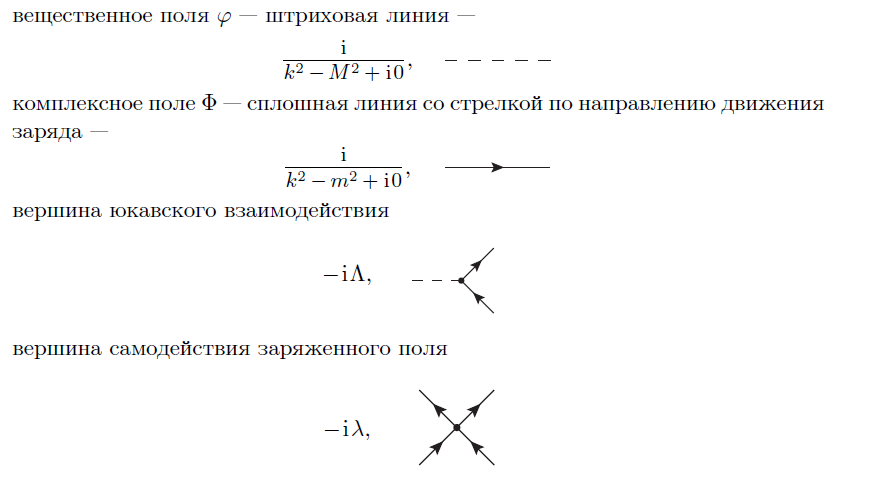
\includegraphics[width=1\linewidth]{pic/feym2}
	\caption{}
	\label{fig:feym2}
\end{figure}






Вершина, как мы убедились, получаются из затравочного действия путем дифференцирования лагранжиана $\mathcal{L}_{\text {int }}$ по полям и домножением на мнимую
единицу. Внешним линиям в конечном состоянии отвечают следуюшие моды:


заряженная частица - отрицательно частотная мода поля $\hat{\Phi}^{\dagger}$, 

заряженная античастица - отрицательно частотная мода поля $\hat{\Phi}$, 

нейтральная частица - отрицательно частотная мода поля $\hat{\varphi}$.





Внешним линиям в начальном состоянии отвечают следующие моды:
заряженная античастица - положительно частотная мода поля $\hat{\Phi}^{\dagger}$, заряженная частица - положительно частотная мода поля $\hat{\Phi}$, нейтральная частица 
- положительно частотная мода поля $\hat{\varphi}$. Для скалярных частиц 
в принятой релятивистски ковариантной нормировке состояний все эти моды в координатном представлении отвечают 
волнам де Бройля с соответствующей прескрипцией для импульсов   и энергий в  начальных и конечных состояниях, 
чтобы выполнялся закон сохранения 4 импульса. В импульсном же 
представлении эти моды оказываются равными
1. Однако понимание того, как они были получены, упростит нам задачу в случае полей с ненулевым спином, когда моды - это многокомпонентные строки или столбцы, а не единицы.

При наличии в диаграмме петель закон сохранения 4-импульса приводит к дополнительному интегрированию по 4-импульсу, который может принимать произвольные значения,
$$
\int \frac{\mathrm{d}^{4} p}{(2 \pi)^{4}}
$$
для каждой петли. Подчеркнем, что при наличии тождественных полей необходимо учесть симметрийный фактор: для внешних полей провести симметризацию по тождественным частицам и сосчитать варианты прескрипции 4-импульсов этим полям, для внутренних линий сосчитать число графических вариантов возникновения одних и тех же диаграмм по заданному набору линий и вершин. Пример расчета симметрийного фактора мы видели в теории кубического самодействия нейтрального поля.

И наконец, повторим, как связана амплитуда с дифференциальной шириной распада частицы массой $M$ с 4 -импульсм $p$



$$
\mathrm{d} \Gamma=\frac{|\mathfrak{M}|^{2}}{2 M} \mathrm{~d} \mathfrak{p}_{f}
$$
где релятивистски инвариантный фазовый объем частиц в конечном состоя-
нии
$$
\mathrm{d} \mathfrak{p}_{f}=(2 \pi)^{4} \delta\left(p-\sum_{n=1}^{n_{f}} k_{(n)}\right) \prod_{n=1}^{n_{f}} \frac{\mathrm{d}^{3} k_{(n)}}{2 E_{(n)}}
$$
и дифференциальным сечением рассеяния частиц с 4-импульсами $p$ и $\tilde{p}$
$$
\mathrm{d} \sigma=\frac{|\mathfrak{M}|^{2}}{4 \sqrt{(p \cdot \tilde{p})^{2}-m^{2} \tilde{m}^{2}}} \mathrm{~d} \mathfrak{p}_{f}
$$
где фазовый объем в конечном состоянии
$$
\mathrm{d} \mathfrak{p}_{f}=(2 \pi)^{4} \delta\left(p+\tilde{p}-\sum_{n=1}^{n_{f}} k_{(n)}\right) \prod_{n=1}^{n_{f}} \frac{\mathrm{d}^{3} k_{(n)}}{2 E_{(n)}}
$$
Отметим, что эти правила относятся к случаю, когда одноточечная функция Грина поля равна нулю. Однако, легко сообразить, что ненулевое


вакуумное значение поля $v=\langle 0|\hat{\varphi}(x)| 0\rangle$ отвечает просто случаю внешнего поля с нулевым импульсом. Такую внешнюю линию обычно изображают с символом $\otimes$ на конце. При этом вершины взаимодействия внешнего вакуумного поля легко определить, если в исходном лагранжиане произвести замену поля, скажем, $\varphi \mapsto v+\varphi$, так что новое поле уже не имеет вакуумного среднего.




























\end{ttask}



\begin{ttask}\textbf{16.}$^{C}$ 

Вывести уравнения Швингера–Дайсона и графическое представление для двухточечной вершинной функции для массивного скалярного поля с самодействием $\lambda \phi^{4} / 4 ! .$ 
Записать правила Фейнмана.





Правила Фейнмана:


1. точный пропагатор дается суммой всех связных диаграмм 


2. каждой вершине отвечает $ -i \lambda \int d^4 x $


3. Свободный пропагатор
$ D_0^F(x,y)=\int \frac{d^4k}{(2\pi)^4} \frac{e^{ik (x-y)}}{k^2-m^2+i\varepsilon} $


4. Комбинаторные множители.













\end{ttask}






\begin{ttask}\textbf{17. }$^{C}$ 

Доказать, что число петель $N_{L}$ В диаграмме с $N_{V}$ степенями действия взаимодействия $V,$ Числом связных компонент диаграммы $N_{c}$ и числом внутренних линий $N_{I}$ определяется соотношением
$$
N_{L}=N_{I}+N_{c}-N_{V}
$$
Привести примеры одно- и двухпетлевых диаграмм с одно- и двухсвязными компонентами в теории с взаимодействием $V \sim \lambda \phi^{4}$




Внутренняя линия добавляет $ \int d^4 x$, а петля снимает.

Для одной связной петли $ N_V=N_I-N_L+1 $


Поэтому для нескольких: $ \sum N_v=\sum N_I - \sum N_L +N_C = N_v=N_I-N_L+N_C $






А также верно следующее:




Амплитуду квантовых переходов при наличии взаимодействий
$$
\hat{Z}(j)=\int \mathcal{D} \varphi \exp \left\{
\frac{\mathrm{i}}{\hbar}\left(S_{0}(\varphi)+j_{x^{\prime}} 
\varphi_{x^{\prime}}\right)
+
\frac{\mathrm{i}}{\hbar} S_{\mathrm{int}}(\varphi)\right\}
$$
можно выразить с помощью действия оператора поля на функционал, построенный для свободных полей,
$$
\hat{Z}(j)=\exp \left\{\frac{\mathrm{i}}{\hbar} S_{\mathrm{int}}\left(-\mathrm{i} \hbar \frac{\delta}{\delta j}\right)\right\} 
\int \mathcal{D} \varphi 
\exp \left\{
\frac{\mathrm{i}}{\hbar}\left(
S_{0}(\varphi)
+
j_{x^{\prime}} \varphi_{x^{\prime}}
\right)
\right\}
$$


Этот функционал позволяет найти общее соотношение для числа петель, 
степени возмущения и числа внутренних линий в связной диаграмме. 

Действительно, если $N_{V}-$ степень вклада возмущения в функцию Грина, 
и значит, $N_{V}$ - это число внутренних вершин в диаграмме, 
то вклад вершин в число 
интегрирований по координатам равен $N_{V}$ (vertex, number of vertecies).

Если в диаграмме есть внутренняя линия, то она соединяет 2 точки, т. е. 
каждой внутренней линии отвечает одно интегрирование по координатам на конце внутренней линии, 
так что при наличии $N_{I}$ внутренних линий (internal lines) $N_{I}$ интегрирований относятся именно к этим линиям, 
и нужно добавить еще одну начальную точку, так что при последовательном счете, 
если рассматривать связную цепочку внутренних линий, 
имеется $N_{I}+1$ число интегрирований в цепочке. 

При этом, поскольку внутренняя линия соединяет именно вершины, 
по сути мы полагаем, что в диаграмме столько же и вершин.

Однако если диаграмма связная, то некоторые начальные и конечные точки в цепочке внутренних линий могут совпасть. 

Каждое такое совпадение означает наличие замкнутой петли. 


Число петель $N_{L}$ (loop, number of loops) определяет число точек посчитанных дважды, так что общее число интегрирований 
по внутренним вершинам или просто число вершин в действительности равно
$$
N_{V}=N_{I}+1-N_{L}, 
\quad 
N_{L}=N_{I}+1-N_{V}
$$
В справедливости данной формулы читатель может наглядно убедиться 
на примере четырех- и двухточечной функции Грина в теории «фи-в-четвертой», как это показано на рис.  




\begin{figure}[H]
	\centering
	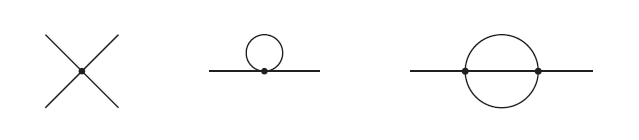
\includegraphics[width=1\linewidth]{pic/petly}
	\caption{}
	\label{fig:petly}
\end{figure}





















\end{ttask}








\begin{ttask}\textbf{18} $^{C}$ 
	
Доказать, что разложение связных Диаграмм по петлям совпадает с разложением по постоянной Планка $\hbar$



Заметим, что связные функции   Грина $ \mathrm{i} G(j) / \hbar  $ 
с   фиксированным числом петель получаются суммированием диаграмм с $N_{V}$ степенями возмущения и 
$N_{I}$ внутренними линиями, причем каждое возмущение дает фактор $1 / \hbar,$ 
а каждая внутренняя линия отвечает обратному оператору на квадратичном по траектории свободном действии, 
т. е. вносит фактор $\hbar(\mathrm{cm} .$ связь связной двухточечной функции Грина со связной частью двухточечной функции Грина 
для амплитуды вероятности $Z(j)$ ). 
В итоге связные функции Грина с петлями имеют следующий масштаб по $\hbar:$
$$
\left.\frac{1}{\hbar} G^{(L)} \sim \sum_{N_{V}, N_{I}}\left(\frac{1}{\hbar}\right)^{N_{V}} \hbar^{N_{I}}\right|_{N_{L} \text { fixed }} \sim \hbar^{N_{L}-1}
$$
Таким образом, разложение связных функций Грина по петлям совпадает с разложением по степеням $\hbar !$ 
Это означает, что в классическом пределе $\hbar \rightarrow 0$ среди связных диаграмм остаются только диаграммы без петель или, как говорят, древесные диаграммы.
































\end{ttask}













\clearpage
\part{Второе задание}


\section{упражнения}

\begin{task}\textbf{8.}$^{C}$ 
	
	Пользуясь антикоммутатором, вычислить следы произведений Гамма-матриц Дирака:
$$
\begin{array}{l}
\operatorname{tr}\left(\gamma^{\mu} \gamma^{\nu}\right), 
\quad 
\operatorname{tr}\left(\gamma_{5} \gamma^{\mu}\right), 
\quad 
\operatorname{tr}\left(\gamma_{5} \gamma^{\mu} \gamma^{\nu}\right), 
\quad 
\operatorname{tr}\left(\gamma^{\mu} \gamma^{\nu} \gamma^{\mu^{\prime}}\right) 
\\
\operatorname{tr}\left(\gamma_{5} \gamma^{\mu} \gamma^{\nu} \gamma^{\mu^{\prime}}\right), 
\quad 
\operatorname{tr}\left(\gamma^{\mu} \gamma^{\nu} \gamma^{\mu^{\prime}} \gamma^{\nu^{\prime}}\right), 
\quad 
\operatorname{tr}\left(\gamma_{5} \gamma^{\mu} \gamma^{\nu} \gamma^{\mu^{\prime}} \gamma^{\nu^{\prime}}\right)
\end{array}
$$












\end{task}



\begin{task}\textbf{9.} $^{C}$ 

Доказать, что след нечетного числа гамма-матриц Дирака равен нулю, а для четного $n$ имеет место соотношение редукции
$$
\operatorname{tr}\left(\gamma^{\mu_{1}} \ldots \gamma^{\mu_{n}}\right)=
g^{\mu_{1} \mu_{2}} \operatorname{tr}\left(\gamma^{\mu_{3}} \ldots \gamma^{\mu_{n}}\right)+
g^{\mu_{1} \mu_{3}} \operatorname{tr}\left(\gamma^{\mu_{2}} \gamma^{\mu_{4}} \ldots \gamma^{\mu_{n}}\right)+
\ldots
$$
























\end{task}



\begin{task} \textbf{10.} 

Упростить выражения

$$
\gamma_{\mu} \cancel{p} \gamma^{\mu}, \quad \gamma_{\mu} \cancel{p} \cancel{k} \gamma^{\mu}
$$























\end{task}



\begin{task}\textbf{11}

Рассмотреть тождества Фирца для гамма-матриц Дирака.












\end{task}



\section{задачи}


\begin{ttask} $\mathbf{1 9 .}^{C}$ 

В ведущем порядке теории возмущений квантовой электродинамики вычислить 
дифференциальное и полное сечения элеткрон-позитронной аннигиляции в мюон-антимюон: 
$e^{+} e^{-} \rightarrow \mu^{+} \mu^{-}$









\end{ttask}



\begin{ttask} $\mathbf{2 0 .}^{C}$ 
	
В ведущем порядке теории возмущений квантовой электродинамики вычислить дифференциальное и полное сечения элеткрон-позитронной аннигиляции в пион-антипион, 
считая пионы точечными скалярными частицами: $e^{+} e^{-} \rightarrow \pi^{+} \pi^{-} .$ 
Сравнить распределение по углами в системе центра масс с распределением в случае образования мюонов.














\end{ttask}



\begin{ttask} $\mathbf{2 1 .}^{C}$ 

В ведущем порядке теории возмущений квантовой электродинамики 
вычислить дифференциальное сечение комптоновского рассеяния фотона на электроне: $\gamma e^{-} \rightarrow \gamma e^{-}$























\end{ttask}



\begin{ttask}

$\mathbf{2 2 .}^{C}$ Вычислить сечение рассеяния электронов на мюонном нейтрино
в модели с четырёхфермионном взаимодействием: $e^{-} \nu_{\mu} \rightarrow \nu_{e} \mu^{-}$




































\end{ttask}



\begin{ttask}

23. $^{C}$ Вычислить ширину трёхчастичного распада мюона на электрон и нейтрино: $\mu^{-} \rightarrow e^{-} \bar{\nu}_{e} \nu_{\mu}$


\end{ttask}



\begin{ttask}

$\mathbf{2 4 .}^{C}$ Вычислить время дВухчастичного распада заряженного пиона:
$\pi^{-} \rightarrow \mu^{-} \bar{\nu}_{\mu} .$ Сравнить ширину распада пиона на электрон и мюон.



\end{ttask}



\begin{ttask}

$\mathbf{2 5 .}^{C}$ Вычислить время распада нейтрона: $n \rightarrow p e^{-} \bar{\nu}_{e}$


\end{ttask}



\begin{ttask}

\textbf{26. }$^{*}$ 




Вычислить ширину двухчастичного распада $Z$ -бозона на нейтри$\mathrm{HO}: Z \rightarrow \nu \bar{\nu}$


\end{ttask}



\begin{ttask}

27. $^{C}$ В ведушем порядке теории возмушений КХД вычислить сечение
$\bar{q} q \rightarrow \bar{c} c$


\end{ttask}



\begin{ttask}

В ведущем порядке теории возмущений КХД вычислить сечение рождения очарованных кварков в глюон-глюоннном слиянии: g g  cc. Рассмотреть синглетный и октетный по цвету вклады в сечение. 



















\end{ttask}


















%\printindex

\bibliographystyle{plain}
\bibliography{bibliography}


\end{document}
